\chapter{Literature Review}
\noindent \rule{6.6in}{0.01in}
\vspace{0.2cm}

This chapter reviews the existing literature at the intersection of decentralized machine learning and edge computing, identifying the research gaps that motivate the proposed APSM framework.

\section{Edge Computing and Decentralized ML}
The shift from centralized cloud computing to decentralized edge computing has been driven by the need for ultra-low latency \cite{shi2016edge}. In this environment, Decentralized Function-as-a-Service (DFaaS) allows for dynamic micro-function execution \cite{ciavotta2021edge}. To perform workload forecasting effectively, edge nodes must train Machine Learning models without compromising data privacy or creating single points of failure. 

To address these requirements, Federated Learning (FL) and Gossip Learning (GL) have emerged as leading paradigms. As illustrated in Figure \ref{fig:fl_vs_gl}, Federated Learning relies on a centralized Aggregator Server to merge model weights \cite{mcmahan2017communication}. If this central server fails, the entire learning process collapses. Conversely, Gossip Learning operates on a fully decentralized peer-to-peer mesh. Nodes randomly share model updates directly with their neighbors, merging the received models locally \cite{ormandi2013gossip}. Tundo et al. (2025) demonstrated that GL can be adapted for edge workload forecasting to achieve high accuracy while maintaining unparalleled fault tolerance \cite{tundo2025decentralized}.

\begin{figure}[!ht]
    \centering
    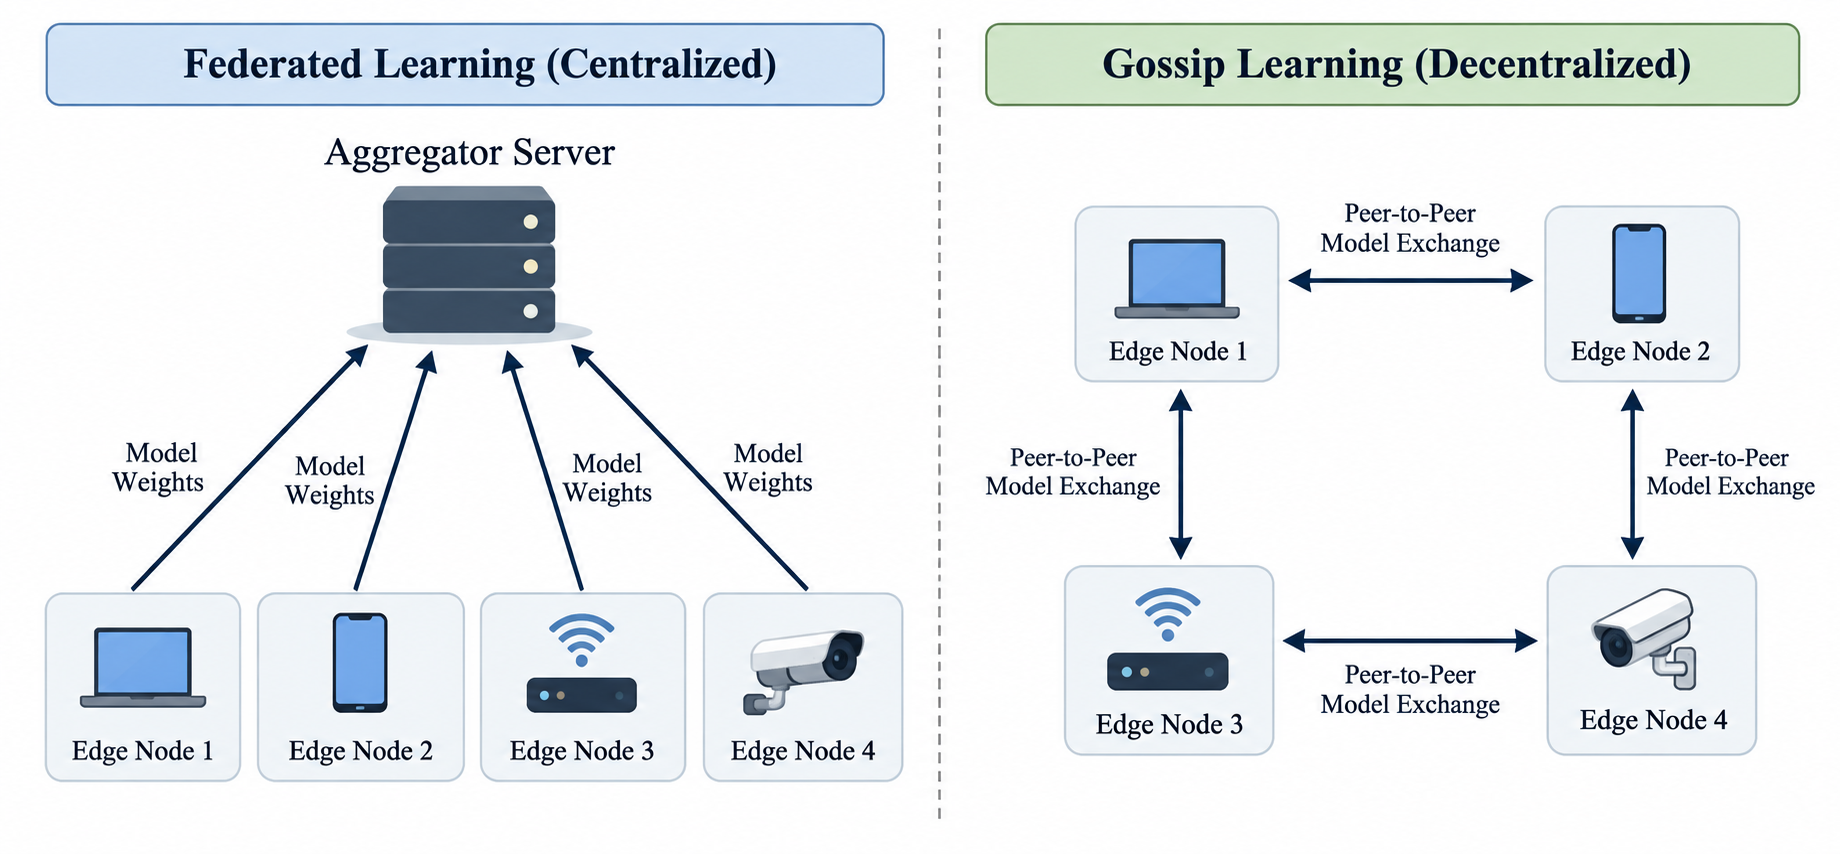
\includegraphics[width=0.6\textwidth]{chapters/figures/fl_vs_gl.png}
    \caption{Comparison of Federated Learning (Centralized Aggregator) and Gossip Learning (Decentralized Peer-to-Peer).}
    \label{fig:fl_vs_gl}
\end{figure}

The visual comparison in Figure \ref{fig:fl_vs_gl} clearly highlights the topological robustness of GL over FL. However, this robustness comes at a severe communication cost.

\section{Research Gaps in Gossip Learning}
Existing literature on Gossip Learning at the edge fails to adequately address the \textit{efficiency} of the knowledge exchange. The standard GL protocol relies on a rigid transmission schedule, leading to massive bandwidth saturation and rapid energy depletion on battery-powered edge devices. Existing protocols do not evaluate the \textit{semantic value} of the data, continuously broadcasting models even when traffic patterns are completely stable.

\section{Evolution towards Agentic AI}
Recent advancements have shown that simply forecasting workloads is insufficient for fully autonomous edge systems. Yao et al. (2025) proposed that dynamic resource orchestration in cloud-native environments requires Multi-Agent Reinforcement Learning (MARL), where heterogeneous agents actively collaborate to allocate resources \cite{yao2025multi}. While Yao et al. demonstrate the power of Agentic AI for reactive scheduling, their models still struggle with delayed feedback and state space explosion. The proposed APSM framework in this thesis bridges this gap: by providing highly efficient, proactive workload forecasts, APSM serves as the critical enabler for stable, forward-looking Agentic AI orchestration at the edge.
